\documentclass[a4paper,12pt,twoside]{memoir}

% Castellano
\usepackage[spanish,es-tabla]{babel}
\selectlanguage{spanish}
\usepackage[utf8]{inputenc}
\usepackage[T1]{fontenc}
\usepackage{lmodern} % Scalable font
\usepackage{microtype}
\usepackage{placeins}
\usepackage{amssymb}
\usepackage{longtable}

\RequirePackage{booktabs}
\RequirePackage[table]{xcolor}
\RequirePackage{xtab}
\RequirePackage{multirow}

% Links
\PassOptionsToPackage{hyphens}{url}\usepackage[colorlinks]{hyperref}
\hypersetup{
	allcolors = {red}
}

% Ecuaciones
\usepackage{amsmath}

% Rutas de fichero / paquete
\newcommand{\ruta}[1]{{\sffamily #1}}

% Párrafos
\nonzeroparskip

% Huérfanas y viudas
\widowpenalty100000
\clubpenalty100000

% Imágenes

% Comando para insertar una imagen en un lugar concreto.
% Los parámetros son:
% 1 --> Ruta absoluta/relativa de la figura
% 2 --> Texto a pie de figura
% 3 --> Tamaño en tanto por uno relativo al ancho de página
\usepackage{graphicx}
\newcommand{\imagen}[3]{
	\begin{figure}[!h]
		\centering
		\includegraphics[width=#3\textwidth]{#1}
		\caption{#2}\label{fig:#1}
	\end{figure}
	\FloatBarrier
}

% Comando para insertar una imagen sin posición.
% Los parámetros son:
% 1 --> Ruta absoluta/relativa de la figura
% 2 --> Texto a pie de figura
% 3 --> Tamaño en tanto por uno relativo al ancho de página
\newcommand{\imagenflotante}[3]{
	\begin{figure}
		\centering
		\includegraphics[width=#3\textwidth]{#1}
		\caption{#2}\label{fig:#1}
	\end{figure}
}

% El comando \figura nos permite insertar figuras comodamente, y utilizando
% siempre el mismo formato. Los parametros son:
% 1 --> Porcentaje del ancho de página que ocupará la figura (de 0 a 1)
% 2 --> Fichero de la imagen
% 3 --> Texto a pie de imagen
% 4 --> Etiqueta (label) para referencias
% 5 --> Opciones que queramos pasarle al \includegraphics
% 6 --> Opciones de posicionamiento a pasarle a \begin{figure}
\newcommand{\figuraConPosicion}[6]{%
  \setlength{\anchoFloat}{#1\textwidth}%
  \addtolength{\anchoFloat}{-4\fboxsep}%
  \setlength{\anchoFigura}{\anchoFloat}%
  \begin{figure}[#6]
    \begin{center}%
      \Ovalbox{%
        \begin{minipage}{\anchoFloat}%
          \begin{center}%
            \includegraphics[width=\anchoFigura,#5]{#2}%
            \caption{#3}%
            \label{#4}%
          \end{center}%
        \end{minipage}
      }%
    \end{center}%
  \end{figure}%
}

%
% Comando para incluir imágenes en formato apaisado (sin marco).
\newcommand{\figuraApaisadaSinMarco}[5]{%
  \begin{figure}%
    \begin{center}%
    \includegraphics[angle=90,height=#1\textheight,#5]{#2}%
    \caption{#3}%
    \label{#4}%
    \end{center}%
  \end{figure}%
}
% Para las tablas
\newcommand{\otoprule}{\midrule [\heavyrulewidth]}
%
% Nuevo comando para tablas pequeñas (menos de una página).
\newcommand{\tablaSmall}[5]{%
 \begin{table}
  \begin{center}
   \rowcolors {2}{gray!35}{}
   \begin{tabular}{#2}
    \toprule
    #4
    \otoprule
    #5
    \bottomrule
   \end{tabular}
   \caption{#1}
   \label{tabla:#3}
  \end{center}
 \end{table}
}

%
% Nuevo comando para tablas pequeñas (menos de una página).
\newcommand{\tablaSmallSinColores}[5]{%
 \begin{table}[H]
  \begin{center}
   \begin{tabular}{#2}
    \toprule
    #4
    \otoprule
    #5
    \bottomrule
   \end{tabular}
   \caption{#1}
   \label{tabla:#3}
  \end{center}
 \end{table}
}

\newcommand{\tablaApaisadaSmall}[5]{%
\begin{landscape}
  \begin{table}
   \begin{center}
    \rowcolors {2}{gray!35}{}
    \begin{tabular}{#2}
     \toprule
     #4
     \otoprule
     #5
     \bottomrule
    \end{tabular}
    \caption{#1}
    \label{tabla:#3}
   \end{center}
  \end{table}
\end{landscape}
}

%
% Nuevo comando para tablas grandes con cabecera y filas alternas coloreadas en gris.
\newcommand{\tabla}[6]{%
  \begin{center}
    \tablefirsthead{
      \toprule
      #5
      \otoprule
    }
    \tablehead{
      \multicolumn{#3}{l}{\small\sl continúa desde la página anterior}\\
      \toprule
      #5
      \otoprule
    }
    \tabletail{
      \hline
      \multicolumn{#3}{r}{\small\sl continúa en la página siguiente}\\
    }
    \tablelasttail{
      \hline
    }
    \bottomcaption{#1}
    \rowcolors {2}{gray!35}{}
    \begin{xtabular}{#2}
      #6
      \bottomrule
    \end{xtabular}
    \label{tabla:#4}
  \end{center}
}

%
% Nuevo comando para tablas grandes con cabecera.
\newcommand{\tablaSinColores}[6]{%
  \begin{center}
    \tablefirsthead{
      \toprule
      #5
      \otoprule
    }
    \tablehead{
      \multicolumn{#3}{l}{\small\sl continúa desde la página anterior}\\
      \toprule
      #5
      \otoprule
    }
    \tabletail{
      \hline
      \multicolumn{#3}{r}{\small\sl continúa en la página siguiente}\\
    }
    \tablelasttail{
      \hline
    }
    \bottomcaption{#1}
    \begin{xtabular}{#2}
      #6
      \bottomrule
    \end{xtabular}
    \label{tabla:#4}
  \end{center}
}

%
% Nuevo comando para tablas grandes sin cabecera.
\newcommand{\tablaSinCabecera}[5]{%
  \begin{center}
    \tablefirsthead{
      \toprule
    }
    \tablehead{
      \multicolumn{#3}{l}{\small\sl continúa desde la página anterior}\\
      \hline
    }
    \tabletail{
      \hline
      \multicolumn{#3}{r}{\small\sl continúa en la página siguiente}\\
    }
    \tablelasttail{
      \hline
    }
    \bottomcaption{#1}
  \begin{xtabular}{#2}
    #5
   \bottomrule
  \end{xtabular}
  \label{tabla:#4}
  \end{center}
}



\definecolor{cgoLight}{HTML}{EEEEEE}
\definecolor{cgoExtralight}{HTML}{FFFFFF}

%
% Nuevo comando para tablas grandes sin cabecera.
\newcommand{\tablaSinCabeceraConBandas}[5]{%
  \begin{center}
    \tablefirsthead{
      \toprule
    }
    \tablehead{
      \multicolumn{#3}{l}{\small\sl continúa desde la página anterior}\\
      \hline
    }
    \tabletail{
      \hline
      \multicolumn{#3}{r}{\small\sl continúa en la página siguiente}\\
    }
    \tablelasttail{
      \hline
    }
    \bottomcaption{#1}
    \rowcolors[]{1}{cgoExtralight}{cgoLight}

  \begin{xtabular}{#2}
    #5
   \bottomrule
  \end{xtabular}
  \label{tabla:#4}
  \end{center}
}



\graphicspath{ {./img/} }

% Capítulos
\chapterstyle{bianchi}
\newcommand{\capitulo}[2]{
	\setcounter{chapter}{#1}
	\setcounter{section}{0}
	\setcounter{figure}{0}
	\setcounter{table}{0}
	\chapter*{#2}
	\addcontentsline{toc}{chapter}{#2}
	\markboth{#2}{#2}
}

% Apéndices
\renewcommand{\appendixname}{Apéndice}
\renewcommand*\cftappendixname{\appendixname}

\newcommand{\apendice}[1]{
	%\renewcommand{\thechapter}{A}
	\chapter{#1}
}

\renewcommand*\cftappendixname{\appendixname\ }

% Formato de portada
\makeatletter
\usepackage{xcolor}
\newcommand{\tutor}[1]{\def\@tutor{#1}}
\newcommand{\course}[1]{\def\@course{#1}}
\definecolor{cpardoBox}{HTML}{E6E6FF}
\def\maketitle{
  \null
  \thispagestyle{empty}
  % Cabecera ----------------
\noindent
\includegraphics[width=\textwidth]{cabecera}\vspace{1cm}%
  \vfill
  % Título proyecto y escudo informática ----------------
  \colorbox{cpardoBox}{%
    \begin{minipage}{.8\textwidth}
      \vspace{.5cm}\Large
      \begin{center}
      \textbf{TFG del Grado en Ingeniería Informática}\vspace{.6cm}\\
      \textbf{\LARGE\@title{}}
      \end{center}
      \vspace{.2cm}
    \end{minipage}

  }%
  \hfill\begin{minipage}{.20\textwidth}
    
\includegraphics[width=\textwidth]{escudoInfor}
  \end{minipage}
  \vfill
  % Datos de alumno, curso y tutores ------------------
  \begin{center}%
  {%
    \noindent\LARGE
    Presentado por \@author{}\\ 
    en Universidad de Burgos \\ \@date{}\\
    Tutor: \@tutor{}\\
  }%
  \end{center}%
  \null
  \cleardoublepage
  }
\makeatother

\newcommand{\nombre}{Roberto Fabián Delgado Pense} %%% cambio de comando

% Datos de portada
\title{Backend como microservicio para aplicación móvil de  Esclerosis Múltiple}
\author{\nombre}
\tutor{D. Pedro Renedo Fernández}
\date{\today}

\begin{document}

\maketitle


\newpage\null\thispagestyle{empty}\newpage


%%%%%%%%%%%%%%%%%%%%%%%%%%%%%%%%%%%%%%%%%%%%%%%%%%%%%%%%%%%%%%%%%%%%%%%%%%%%%%%%%%%%%%%%
\thispagestyle{empty}


\noindent
\includegraphics[width=\textwidth]{cabecera}\vspace{1cm}

\noindent D. Pedro Renedo Fernandez, profesor del departamento de Ingeniería Informática del área de Lenguajes y Sistemas Informáticos.

\noindent Expone:

\noindent Que el alumno D. \nombre, con documento de identidad uruguayo nro. 3.976.767-7 y Pasaporte nro. D263709, ha realizado el Trabajo final de Grado en Ingeniería Informática titulado "Backend como microservicio para aplicación móvil de Esclerosis Múltiple". 

\noindent Y que dicho trabajo ha sido realizado por el alumno bajo la dirección del que suscribe, en virtud de lo cual se autoriza su presentación y defensa.

\begin{center} %\large
En Burgos, {\large \today}
\end{center}

\vfill\vfill\vfill

% Author and supervisor
% \begin{minipage}{0.45\textwidth}
% \begin{flushleft} %\large
% Vº. Bº. del Tutor:\\[2cm]
% D. nombre tutor
% \end{flushleft}
% \end{minipage}
% \hfill
% \begin{minipage}{0.45\textwidth}
% \begin{flushleft} %\large
% Vº. Bº. del co-tutor:\\[2cm]
% D. nombre co-tutor
% \end{flushleft}
% \end{minipage}
\hfill

\vfill

% para casos con solo un tutor comentar lo anterior
% y descomentar lo siguiente
Vº. Bº. del Tutor:\\[2cm]
D. Pedro Renedo Fernández


\newpage\null\thispagestyle{empty}\newpage

\frontmatter

% Abstract en castellano
\renewcommand*\abstractname{Resumen}
\begin{abstract}
El presente proyecto se enfocó en el desarrollo del backend para una aplicación móvil de asistencia para personas afectadas por la Esclerosis Múltiple (EM) que les ayudase a navegar por el sistema de salud desde el momento del diagnostico, así como para autogestionar la enfermedad.
El backend fue desarrollado en base a lenguaje Golang y Python, con el objetivo de ofrecer diversidad de funciones tales como chatbot, diario de control de síntomas y medicación, recordatorios, artículos, entre otros. Se emplearon tecnologías y plataformas como PostgreSQL, Postman, Docker, Swagger, FAISS, GitHub, Jira, Visual Code Studio y SonarQube, aplicando, durante todo el proceso, la metodología SCRUM, como marco de trabajo ágil para la gestión del proyecto.
\end{abstract}

\renewcommand*\abstractname{Descriptores}
\begin{abstract}
Esclerosis Múltiple, EM, aplicación móvil, backend, Golang, Python, FAISS, SonarQube, Scrum, Docker, seguimiento del paciente, autonavegación, EMUR.\end{abstract}

\clearpage

% Abstract en inglés
\renewcommand*\abstractname{Abstract}
\begin{abstract}
This project focused on the development of the backend for a mobile application to offer support for people affected by
Multiple Sclerosis (MS) to help them navigate the health system from diagnosis, as well as to support self-management of the disease. The backend was developed based on Golang language and Python, with the aim of providing diversity of functions such as chatbot, symptom and medication control diary, reminders, articles, among others. A number of technologies and platforms were used, such as PostgreSQL, Postman, Docker, Swagger, FAISS, GitHub, Jira, Visual Code Studio and SonarQube, applying, throughout the process, the SCRUM methodology, as an agile framework for the management of project.
\end{abstract}

\renewcommand*\abstractname{Keywords}
\begin{abstract}
Multiple Sclerosis, MS, mobile application, backend, Golang, Python, FAISS, SonarQube, Scrum, Docker, patient follow-up, self-navigation, EMUR.
\end{abstract}

\clearpage

% Indices
\tableofcontents

\clearpage

\listoffigures

\clearpage

\listoftables
\clearpage

\mainmatter
\capitulo{1}{Introducción}

\subsection{Encuadre del TFG}
La presente entrega se enmarca en la formación de Grado en Ingeniería Informática impartida por la Universidad de Burgos de España, constituyendo la última instancia evaluativa requerida para la aprobación de la misma.
En tanto trabajo final de grado (TFG), su propósito radica en propiciar la articulación de los contenidos abordados conforme avanzó el ciclo educativo y valorar la incorporación de las competencias adquiridas para el egreso.

Amerita mencionar que la redacción presentada a continuación está realizada en castellano rioplatense, un derivación de la lengua española hablada en algunos países de latinoamérica, puesto que mi nacionalidad y lugar de residencia es Uruguay.

\subsection{Introducción al TFG}
Una aplicación móvil, también conocida como app, por el vocablo application en idioma inglés, es un software diseñado para ser utilizado en dispositivos móviles como smartphones o tablets, bien sean de sistemas operativos iOS o Android. Estas aplicaciones pueden ser descargadas e instaladas desde tiendas virtuales como Google Play o Apple Store y ofrecen una amplia variedad de funciones y servicios. Asimismo, pueden ser clasificadas en diferentes categorías; a saber: juegos, redes sociales, productividad, entre otras. De esta forma, las aplicaciones móviles pueden ser utilizadas en una amplia variedad de campos tales como la educación, la salud, el comercio electrónico y el entretenimiento.

Dentro del ámbito de la salud, las aplicaciones móviles han revolucionado la forma en que los pacientes interactúan con los proveedores de atención médica y gestionan su propia salud. Estas aplicaciones pueden ser utilizadas para diversos propósitos, desde el seguimiento de la administración de medicamentos hasta la monitorización de la actividad física y la gestión de enfermedades crónicas. Ello permite, a pacientes y profesionales, tener acceso a información y servicios en línea, siendo más eficientes, por lo que representan una herramienta muy valiosa y especialmente útil para personas con enfermedades de curso crónico como lo es la Esclerosis Múltiple (en adelante EM), que a menudo necesitan navegar por un sistema de atención sanitaria complejo y fragmentado a lo largo de las diferentes etapas de su ciclo vital.

La EM es una enfermedad neurológica que afecta al Sistema Nervioso Central, de origen multicausal, pero cuyo factor desencadenante aún no ha sido descubierto. Se trata de una enfermedad inflamatoria, autoinmune, y potencialmente discapacitante.

Se ha identificado que la progresión deviene con el paso del tiempo en todos los tipos de EM desde las primeras etapas de la enfermedad, incluso si el individuo no experimenta síntomas, siendo algunos de los más frecuentes:

\begin{itemize}
\tightlist
\item
    visión doble y/o borrosa 
\item
    dificultades en el habla
\item
    parestesias 
\item
    espasticidad 
\item
    afectación cognitiva     
\item   
    entumecimiento 
\item   
    ataxia 
\item   
    fatiga
\item   
    dolores musculares
\item   
    pérdida de fuerza
\item   
    disminución de la sensibilidad
\item   
    afectación a nivel urológico
\end{itemize}

El diagnóstico de una patología crónica y de constante progresión, así como la amplia diversidad de síntomas y la incertidumbre de la evolución, son aspectos que suelen tener un impacto multidimensional (biológico, cognitivo, psicoemocional, socio-ecológico, espiritual) significativo en la calidad de vida de las personas que conviven con EM, quienes suelen enfrentar muchos desafíos en el proceso de diagnóstico, tratamiento y seguimiento de su enfermedad. 

Desde el momento en que son diagnosticados, los pacientes pueden necesitar coordinar citas con múltiples especialistas, obtener recetas y medicamentos, y conocer en profundidad los servicios ofrecidos por su prestador de salud. Asimismo, a medida que la enfermedad progresa, pueden necesitar acceder a diferentes tipos de terapias y tratamientos. 

Esta enfermedad, que afecta a más de 2.8 millones de personas en todo el mundo, presenta, en Uruguay, el índice de prevalencia más alto de Latinoamérica  y, reporta 94 casos nuevos por año en el país, de acuerdo al estudio multicéntrico EMELAC culminado en 2022.

En este contexto, el desarrollo de una aplicación móvil específica para ayudar a las personas con EM a moverse por el sistema sanitario puede ser una herramienta muy efectiva. Esta aplicación podría ser utilizada para integrar diferentes servicios de salud, como citas médicas, pruebas diagnósticas, tratamientos y seguimiento sintomático, en una sola plataforma. De esta manera, los pacientes podrían acceder a los servicios de salud necesarios de manera más rápida y eficiente, lo que mejoraría su calidad de vida.

En relación con lo anterior, el backend de la aplicación que se propone en el presente proyecto permitirá a las personas con EM acceder, de manera más eficiente, a información respecto a su enfermedad y a los recursos necesarios para navegar por el sistema sanitario, asi como también los dispositivos existentes en la matriz de protección social.

Por lo tanto, y en definitiva, el desarrollo de una aplicación móvil focalizada en la experiencia del enfermar con EM, configura una oportunidad única para optimizar la calidad de vida de las personas afectadas por esta patología, asi como también de toda la sociedad uruguaya.

Esta aplicación tiene potencial para ser replicable y escalable a otras patologías así como también a otros contextos socio-económicos, culturales y geográficos, constituyendo una herramienta muy valiosa para integrar diferentes funcionalidades relativas a la salud en una sola plataforma. Asimismo, sienta el terreno fértil para la recolección de datos e información relevante que permita a tomadores de decisión mapear y perfilar la comunidad de personas con EM en el país para desarrollar soluciones acorde a sus necesidades.



\capitulo{2}{Objetivos del proyecto}

Con este proyecto se pretende desarrollar el backend de una futura aplicación móvil, a llamar \emph{RedEM}, focalizada en la experiencia de enfermar para personas afectadas por la EM constituyendo un mapa de autonavegación que les permita hacer uso del sistema sanitario y autogestionar su patología.

Para ello, se plantean los siguientes objetivos funcionales mínimos que el backend a desarrollar deba cumplir:

\section{Objetivos generales}

\begin{itemize}
    \item Ser eficiente y eficaz para el procesamiento y manipulación de datos.
    \item Presentar una sólida, coherente y confiable lógica de negocio. 
    \item Ponderar la seguridad, privacidad e integridad de la información sensible que los usuarios comparten.
    \item Permitir una robusta escalabilidad y rendimiento del sistema.
    \item Permitir que el sistema se integre con servicios internos y externos tales como APIs.
    \item Habilitar un monitoreo y un registro de errores que haga al sistema tolerante a fallos. 
\end{itemize}

\section{Objetivos personales}
\begin{itemize}
\item incluir un chatbot que permita visualizar el funcionamietno de la api por la complejidad 
    \item Incorporar los conceptos fundamentales y aplicaciones del lenguaje de programación Golang para el desarrollo de APIs.
    \item Comprender el funcionamiento de los servidores web y cómo desplegar proyectos desarrollados con el lenguaje Golang.
    \item Aprender a diseñar e implementar APIs RESTful acorde a los estándares de la industria y los principios de escalabilidad.
    \item Adquirir conocimientos sobre el manejo de bases de datos y sistemas de almacenamiento en la nube, y cómo realizar las integraciones con el backend de una aplicación móvil.
    \item Profundizar en el conocimiento de tecnologías y herramientas relacionadas con la seguridad de aplicaciones móviles y servidores.
    \item Robustecer el conocimiento en cuanto al uso de sistema de control de versiones Git, a través de la plataforma GitHub, para trabajar de manera eficiente en proyectos de desarrollo de software en equipo.
   \item Aprehender a utilizar software para la planificación y ejecución del trabajo de desarrollo de software mediante el uso de la metodología SCRUM.
    \item Conocer cómo utilizar el procesador de textos \LaTeX\ para la creación de documentos técnicos y científicos de alta calidad, como la memoria del presente proyecto.   
\end{itemize} 

\newcommand{\graybox}[2]{%
    \colorbox{gray!20}{%
        \parbox{\dimexpr\linewidth-2\fboxsep}{%
            \colorbox{black}{\textcolor{white}{\textbf{\makebox[\dimexpr\linewidth-2\fboxsep]{#1}}}}\vspace{4pt}%
            \hspace{\parindent}#2%
        }%
    }%
}

\graybox{A considerar:}{\\Debido a que el TFG pondera únicamente el desarrollo del backend, no así de la aplicación \emph{RedEM}, la visibilidad o testing del proyecto queda restringida. \\Por tal motivo se emplea la plataforma Postman para que el comité evaluador se sirva probar el funcionamiento de las APIs, tanto del backend como del chatbot, conforme figura en el Manual de Usuario. \\
Amerita explicitar, además, que para las APIs de backend los datos son ficticios, mientras que en el caso del chatbot, la información es extraída del sitio web de la Asociación.}



            



\section{Análisis de mercado}
Para la creación del presente proyecto se consideró la posible existencia de otras aplicaciones de similares características a nivel global. Por tanto, en este apartado se expondrá información relativa a: población objetivo, competencia y antecedentes, y análisis FODA en base a la información relevada.

\subsection{Público objetivo y perfiles de usuario}
\emph{RedEM} es una aplicación dirigida a los principales grupos afectados e involucrados en la EM, que sería: personas con EM, allegados y familiares, personal sanitario de carácter multidisciplinar.

\begin{itemize}
    \item 
    \textbf{Personas con EM:} Los pacientes presentan una amplia gama de síntomas que pueden variar de un individuo a otro tanto en frecuencia, como en tipo e intensidad. En tal sentido, cada paciente tendrá una serie de necesidades diferentes requiriendo un tratamiento y seguimiento particular, lo que debe ser considerado dentro del diseño de la aplicación móvil y su usabilidad.
    \item 
    \textbf{Allegado y familiares:} Ante el diagnóstico de EM, el entorno del paciente se ve afectado, en especial aquellas personas que asumen el rol de cuidadores. Éstos tienen, a su vez, una serie de necesidades que también debe ser cubiertas o que ameritan una solución, como por ejemplo: consejos para el cuidador del paciente, primeros auxilios en caso de emergencia, apoyo emocional, o cualquier otra necesidad que pueda surgir.
   \item 
   \textbf{Personal sanitario multidisciplinar:} Por ser una enfermedad neurológica que afecta el funcionamiento del sistema nervioso central, puede generar síntomas funcionales y estructurales que repercuten en diversas áreas del organismo siendo imprescindible un abordaje integral con la participación de diversos especialistas como ser: neurólogos, fisioterapeutas, terapista ocupacional, psicólogos, sexólogos, entre otros.  
\end{itemize} 


\subsection{Competencia/Antecedentes}
Existen diversas aplicaciones que buscan ayudar a potenciar la autonomía personal de los pacientes con EM. No obstante, la mayoría de ellas se centran en consejos y ejercicio físicos, más no tienen en cuentan la comunicación con especialistas ni el control y seguimiento de la enfermedad y su tratamiento. A este respecto, el análisis de la competencia se enfocó en la búsqueda de aplicaciones que cumplieron con el objetivo del presente proyecto para, posteriormente, compararlas con \emph{RedEM}. A continuación, se describen las cuatro aplicaciones que se encontraron:

\subsubsection{Cleo}
Cleo es una app móvil, para iOS y Android, desarrollada por la compañía Biogen, y cuyo objetivo es brindar acompañamiento a los pacientes de EM. Para ello le permite a los usuarios establecer diálogos directos, mediante chats, con servicios de enfermería especializados con la EM para resolver dudas o solicitar apoyo, al mismo tiempo que proporciona otras herramientas como contenido de valor en forma de consejos, noticias y artículos con información de interés.

\begin{figure}[h]
    \centering
    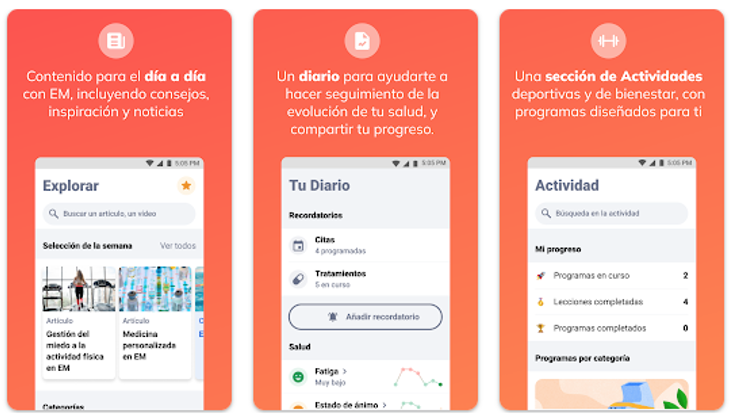
\includegraphics[width=0.7\textwidth]{img/mercado/cleo.png}
    \caption{Cleo App.} \label{Img:Cleo+App}
\end{figure} 

Por otro lado, también dispone de un diario para llevar un control y registro de la salud del paciente, los síntomas que ha presentado a lo largo del día, y su estado de ánimo, que luego pueda compartir con el personal sanitario. Asimismo, propone planes de ejercicio físico adaptado, y un sistema de alarmas y recordatorios para citas médicas y tratamientos.

A pesar de sus bondades, esta aplicación no permite ser descargada en Latinoamérica y, al tratarse de una herramienta digital creada por una farmacéutica, los datos allí cargados terminan siendo propiedad de la misma.

\subsubsection{ME - Multiple Esclerosis}

ME es un app móvil disponible en iOS y Android, desarrollada por Novartis. Su objetivo principal en facilitar el seguimiento y control de los síntomas del paciente, para lo cual cuenta con tres funciones básica. La primera de ellas, un plan de ejercicios diseñado para optimizar la movilidad y capacidad cognitiva.

Luego, la aplicación cuenta con una sección para el registro de datos diarios, semanales o mensuales, referentes a las consultas médicas y horarios de tratamiento, en la que podrán también configurar alarmas y recordatorios; y un cuerpo humano interactivo en el que el usuario podrá indicar las partes de su cuerpo donde presenta síntomas. Por otra parte, sirve también de apoyo al personal de salud quienes podrán llevar un seguimiento a partir de la información recogida por la app.

\begin{figure}[h]
    \centering
    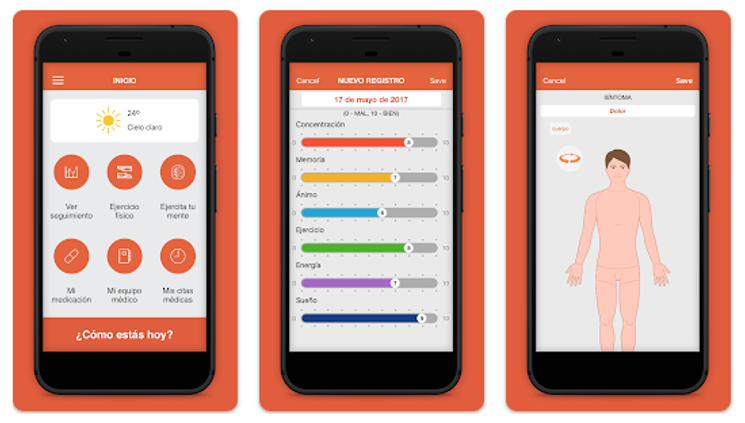
\includegraphics[width=0.5\textwidth]{img/mercado/me.png}
    \caption{ME App} \label{Img:ME+App}
\end{figure} 

Tal como en el caso anterior, está aplicación no puede ser descargada en la región y los datos son propiedad de una empresa farmacéutica. 

\subsubsection{Control EM}

Si bien no fue posible acceder en la actualidad a esta aplicación ni descargarla en la región, en tanto antecedente amerita mencionarla. Control EM era una aplicación para iOS, desarrollada por la Fundación Esclerosis Múltiple Madrid (FEMM) y que, al igual que las anteriores, buscaba ayudar a los pacientes a llevar un control de su enfermedad, su evolución, disponer de información de interés y comunicarse con especialistas. 

\begin{figure}[h]
    \centering
    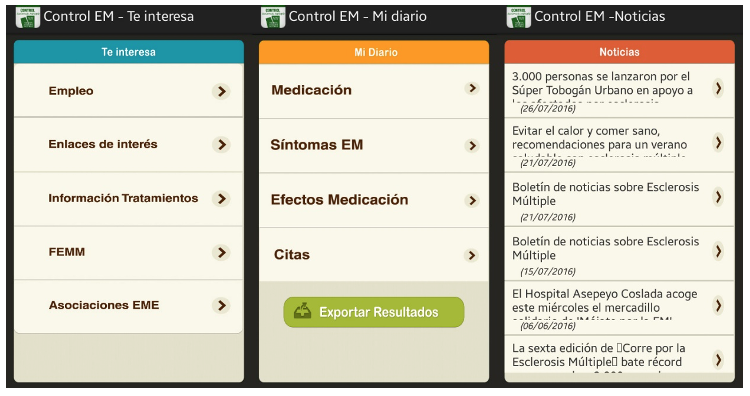
\includegraphics[width=0.5\textwidth]{img/mercado/control_em.png}
    \caption{Control EM App} \label{Img:Control+EM+APP}
\end{figure} 

Contaba con cuatro secciones principales: a) mi diario, en donde el usuario podía anotar su horario de tratamiento, síntomas, efectos de la medicación y citas médicas, para así conocer su evolución a través de gráficas; b) agenda, donde se mostraban las citas anuales vinculadas con la EM, como conferencias; c) noticias, donde se brindaba información sobre la EM; y d) te interesa, que incluía información sobre tratamientos disponibles, empleo, taxis adaptados, y contactos de la FEMM u otras asociaciones.

\subsubsection{Emilyn}

Al igual que el caso anterior, Emilyn sirve como antecedente a nuestros propósitos ya que no fue posible encontrarla activa. Esta aplicación funcionaba como una compañera digital para la persona con EM, permitiéndole llevar un control y registro de los síntomas, crear alertas y recordatorios para la medicación y las citas médicas, guardar y compartir informes médicos, o descubrir potenciales desencadenantes de empujes. Esta aplicación sólo estaba disponible en inglés y no se encontraba habilitada para la región.

\begin{figure}[h]
    \centering
    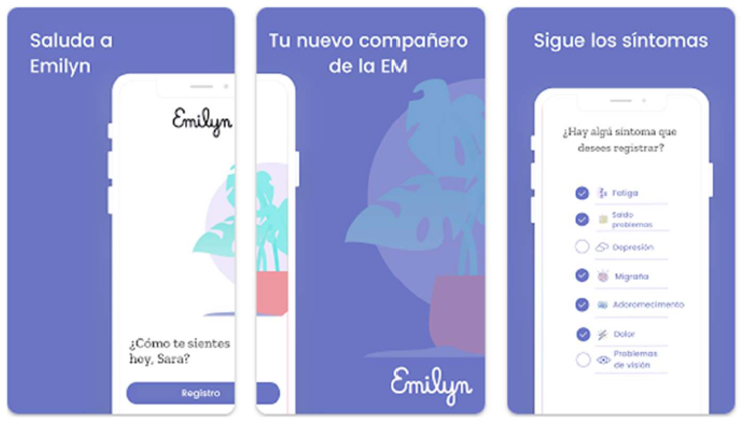
\includegraphics[width=0.5\textwidth]{img/mercado/emylin.png}
    \caption{Emylin App} \label{Img:Emilyn+APP}
\end{figure} 

\subsection{Discusión del estado de mercado para los objetivos del proyecto}
Habiendo analizado las aplicaciones existentes en el mercado que se acercan al objetivo planteado y a las necesidades del presente proyecto, se procede a formular un análisis FODA al respecto de \emph{RedEM}.

\subsection{Análisis FODA}

\begin{tabular}{|c|l|}
\hline
\textbf{Fortalezas} & \parbox{10cm}{
\begin{itemize}
    \item Aplicación gestionada por una organización civil y no la industria farmacéutica, por lo que se erradican conflictos de interés actuales o potenciales.
    \item Contribuye a la creación de un mapa de autonavegación a partir de información proporcionada por la sociedad civil organizada (live-experience), desde una perspectiva holística y multidimensional.
    \item Ofrece al usuario información referida a dispositivos y programas disponibles en la matriz de protección social, asi como recetas alimenticias, sección de preguntas y respuestas, y estado del clima para el cuidado del paciente, en formato de artículos.
    \item El frontend se desarrollará en lenguaje Flutter para permitir ahorrar costos de desarrollo por concepto de portabilidad de código.
    \item El chatbot con IA es algo novedoso y que permite descongestionar la atención telefónica que brinda la Asociación EMUR.
\end{itemize}
} \\
\hline
\textbf{Oportunidades} & \parbox{10cm}{
\begin{itemize}
    \item Permite que los pacientes estén interconectados para sobrellevar la enfermedad, generando comunidad.
    \item La mayoría de la población uruguaya cuenta con smartphones con acceso a internet.
    \item A nivel país se tiene un estable acceso a internet debido a que se cuenta con la infraestructura para ello. 
    \item Tiene potencial para ser replicable y escalable a otras patologías así como también a otros contextos socio-económicos, culturales y geográficos.
    \item Auge de la telemedicina, así como de iniciativas de recolección de resultados y experiencias aportadas por los pacientes (PROMs y PREMs).
\end{itemize}
} \\
\hline
\end{tabular}

\begin{tabular}{|c|l|}
\hline
\textbf{Debilidades} & \parbox{10cm}{
\begin{itemize}
    \item Aún no permite establecer contacto directo con el personal sanitario mediante chat.
    \item La Asociación es pequeña para administrar los contenidos de la aplicación, por lo que requerirá un equipo de gestión de contenidos.
    \item Al tratarse de una Asociación de exiguos ingresos, será un desafío asumir a largo plazo los costos de mantenimiento y difusión.
\end{itemize}
} \\
\hline
\textbf{Amenazas} & \parbox{10cm}{
\begin{itemize}
    \item Baja adopción por parte de los usuarios, debido a que Uruguay presenta una población mayoritariamente envejecida y existe fuga de cerebros.
    \item Aplicaciones de la industria farmacéutica que puedan desarrollarse en la región próximamente, o que sean adaptadas para Latinoamérica. 
    \item Cambios respecto a la normativa vigente en cuanto al uso de datos personales.
\end{itemize}
} \\
\hline
\end{tabular}






\capitulo{3}{Conceptos teóricos}

El propósito de esta sección es establecer un marco de referencia para el proyecto a partir de los conceptos teóricos básicos relacionados con las tecnologías y recursos que se utilizaron a lo largo del mismo.

\section{Aplicación móvil}
Una aplicación móvil es un software diseñado para ser utilizado en dispositivos móviles como smartphones o tablets. Las aplicaciones móviles tienen un mejor rendimiento y acceso a características del dispositivo, mientras que las aplicaciones web son más fáciles de desarrollar y mantener \cite{art:native_apps_vs_mobile_apps}. Sin embargo, el desarrollo de aplicaciones móviles presenta desafíos como la compatibilidad con diferentes dispositivos y sistemas operativos, y la seguridad de los datos \cite{art:challenges_and_best_practices}. En este sentido, el desarrollo de una aplicación móvil es un proceso que se compone de las siguientes etapas:

\begin{itemize}
\item \textbf{Análisis de requerimientos}: En este paso se identifican y documentan las necesidades del cliente y se definen los requerimientos de la aplicación, siendo este análisis una actividad crítica que establece la base para el desarrollo exitoso del software \cite{book:ingenieria_del_software}.

\item \textbf{Diseño de la arquitectura}: En este paso se define la estructura de la aplicación, incluyendo la interacción entre las diferentes partes. Se diseñan la interfaz de usuario, la arquitectura del software y la base de datos. El diseño de la arquitectura es una parte crucial del desarrollo de una aplicación móvil \cite{art:mobile_application_development}.

\item \textbf{Desarrollo de la aplicación}: En este paso se escribe el código y se implementa la aplicación, siguiendo el diseño definido anteriormente. El desarrollo de la aplicación es un proceso iterativo que involucra la implementación, prueba y corrección de errores \cite{art:asana_proceso_desarrollo}. Es el proceso de traducir el diseño en un programa ejecutable \cite{book:ingenieria_software_pearson}.

\item \textbf{Pruebas de la aplicación}: En este paso se realizan pruebas exhaustivas de la aplicación para detectar y corregir errores. Se evalúa la calidad de la aplicación mediante pruebas funcionales y de rendimiento. Las pruebas son una parte fundamental del proceso de desarrollo \cite{book:tipos_pruebas_funcionales}.

\item \textbf{Lanzamiento de la aplicación}: En este paso se lanza la aplicación al mercado. El lanzamiento es un proceso crítico que involucra la promoción y distribución de la aplicación a los usuarios finales \cite{art:asana_proceso_desarrollo}.

\end{itemize}

\section{API}
API es el acrónimo para ‘Application Programming Interface’, con lo cual se hace referencia a un conjunto de reglas, protocolos y herramientas que permiten la comunicación entre diferentes aplicaciones y sistemas de software \cite{art:architectural_styles} para qué estas puedan enviar y recibir datos entre ellas de manera estandarizada y segura. Así, una API es una especificación de cómo se deben comunicar dos componentes de software \cite{book:restful_webservices_allamaraju}. Lo anterior implica que una API es la interfaz de programación de aplicaciones que permite a los desarrolladores acceder y utilizar los datos y funcionalidades de una aplicación sin tener que conocer todos los detalles de su implementación.
En este sentido, las APIs son una de las herramientas más importantes para la creación de aplicaciones web y móviles \cite{art:designing_web_api}. El uso de API se ha vuelto cada vez más popular en los últimos años debido a su capacidad para mejorar la interoperabilidad y la eficiencia en el desarrollo de aplicaciones. Ahora, el desarrollo de una API es un proceso que implica varios pasos y fundamentos teóricos importantes, los cuales se describirán a continuación \cite{art:architectural_styles}:

\begin{itemize}
\item \textbf{Definición de los requisitos}: Antes de comenzar el desarrollo de una API, es importante definir los requisitos que debe cumplir. Esto incluye identificar los casos de uso, las funcionalidades que se necesitan implementar y los tipos de datos que van a ser intercambiados a través de la API.   

\item \textbf{Diseño de la arquitectura}: Una vez que se han definido los requisitos, es necesario diseñar la arquitectura de la API. Esto implica decidir qué tecnologías se van a utilizar, cómo se van a estructurar los componentes de la API y cómo se van a gestionar las peticiones y respuestas.

\item \textbf{Implementación}: Se codifica la lógica de negocio, se crean los endpoints y se configuran los servidores para que puedan manejar las peticiones y respuestas de la API. Por otro lado, la implementación de una API debe ser escalable y capaz de manejar grandes volúmenes de peticiones y respuestas. \cite{art:architectural_styles}.

\item \textbf{Prueba y depuración}: Una vez que la API ha sido implementada, es necesario probarla y depurarla. Esto implica verificar que se cumplen los requisitos, que la API es segura y que funciona correctamente en distintos entornos y situaciones. La seguridad de la API es un aspecto crítico que debe ser tenido en cuenta durante todo el proceso de desarrollo. Es necesario implementar medidas de seguridad como la autenticación y la autorización para proteger los datos y prevenir ataques malintencionados \cite{book:beatiful_code}.

\item \textbf{Documentación}: Finalmente, es importante documentar la API para que los desarrolladores puedan entender cómo utilizarla correctamente. La documentación debe incluir una descripción de los endpoints, los parámetros y los tipos de datos que se pueden intercambiar a través de la API, así como también ejemplos de código para que los desarrolladores puedan entender cómo utilizar la API en su código \cite{book:restful_webservices_richardson}.

\end{itemize}

\section{APIs RESTful}
Una API RESTful (Representational State Transfer) es un conjunto de reglas y restricciones para crear servicios web que sean escalables, flexibles y fáciles de mantener. Utiliza el protocolo HTTP para definir las operaciones y los recursos a los que se accede a través de la API. A este respecto, la arquitectura REST es un estilo arquitectónico que se utiliza para diseñar sistemas distribuidos en la web. Se basa en el uso de recursos identificados por URLs y en la manipulación de estos recursos a través de los métodos HTTP \cite{book:restful_webservices_richardson}.
En términos generales, una API RESTful funciona mediante solicitudes HTTP que se envían a través de Internet. Estas solicitudes pueden ser de diferentes tipos, como GET, POST, PUT, PATCH, DELETE, entre otros, y se utilizan para realizar operaciones específicas en los recursos de la API. Los recursos se identifican mediante URLs, y los datos se transfieren en formato JSON o XML \cite{art:google_app_engine}.
Una API RESTful es una interfaz de programación de aplicaciones que sigue los principios de REST y que permite a los desarrolladores acceder a los recursos de una aplicación a través de Internet \cite{art:architectural_styles}. En este sentido, la arquitectura REST se basa en el principio de que cada recurso de una aplicación debe tener una URL única y que se deben utilizar los métodos HTTP adecuados para acceder a ellos. De esta manera, se consigue una mayor escalabilidad y una mejor separación entre el cliente y el servidor.

\section{JSON}
JSON (JavaScript Object Notation) es un formato de intercambio de datos utilizado para transmitir información estructurada a través de una red por lo que se utiliza principalmente en aplicaciones web y móviles, como por ejemplo en el desarrollo de APIs RESTful, debido a su simplicidad, flexibilidad, ligereza y su capacidad para representar datos estructurados de una manera fácil de entender. 
Otras de sus ventajas, son su facilidad de uso, la capacidad de ser leído por cualquier lenguaje de programación, su tamaño reducido en comparación con otros formatos de intercambio de datos y el hecho de que es un formato abierto y estándar \cite{art:comparision_json_xml}. 
Por otra parte, algunas desventajas son su falta de soporte para algunos tipos de datos complejos y su dependencia de un parser para su interpretación.
En este sentido, JSON es un formato de texto que es completamente independiente de cualquier lenguaje de programación, pero utiliza convenciones que son familiares para los programadores de la familia de lenguajes C, incluyendo Java, JavaScript, Perl, Python, y muchos otros \cite{art:json_media_type}. JSON es una alternativa más ligera y fácil de usar a XML para la transferencia de datos estructurados entre sistemas \cite{art:google_app_engine}.

\section{Git y GitHub}
Git es un sistema de control de versiones distribuido que permite a los programadores gestionar cambios en el código fuente de un proyecto de software de manera colaborativa, mientras que GitHub es una plataforma en línea que se utiliza para alojar repositorios de Git y para facilitar la colaboración en proyectos de software \cite{art:pro_git}.
El funcionamiento de Git se basa en el control de versiones mediante la creación de ramas (branches) que permiten trabajar en diferentes versiones del código de manera independiente y luego fusionarlos. Por su parte, GitHub proporciona herramientas para la gestión de proyectos, como la creación de issues, pull requests y colaboración en equipo.

\section{Base de datos}
Una base de datos es un conjunto de datos interrelacionados, estructurados y organizados que se almacenan en un sistema informático para su uso en una aplicación específica \cite{book:base_de_datos_connolly}. Sus componentes principales son el software de gestión de bases de datos, el hardware (como servidores y discos duros) y los datos en sí mismos \cite{book:base_de_datos_coronel}. 
Las bases de datos se utilizan para almacenar y gestionar grandes cantidades de información  empresarial, científica y personal, por tanto sus aplicaciones son muy variadas y van desde sistemas de gestión de inventarios hasta sistemas financieros y de recursos humanos. El funcionamiento de una base de datos se sustenta en la adición, modificación y eliminación de información a través de un lenguaje de consulta estructurado SQL (Structured Query Language) \cite{book:base_de_datos_ramakrishnan}. Los datos se organizan en tablas y se relacionan entre sí mediante claves primarias y foráneas. 

\section{Docker}
Docker es una plataforma de contenedores de software que permite a los desarrolladores empaquetar y distribuir aplicaciones junto con sus dependencias, de manera consistente y confiable en diferentes entornos, en un paquete portátil llamado contenedor \cite{art:docker_containers}. En este sentido, los contenedores son unidades de software que incluyen todo lo necesario para ejecutar una aplicación, incluidas bibliotecas, dependencias y configuraciones \cite{art:docker_boettinger}. A este respecto, el uso de contenedores Docker puede mejorar la eficiencia del desarrollo de software al permitir la creación de entornos de desarrollo aislados y reproducibles. 
Los componentes principales de Docker son el daemon de Docker, la CLI de Docker y el Docker Hub. El daemon de Docker es el servidor que ejecuta los contenedores, la CLI de Docker es la herramienta de línea de comandos que se utiliza para interactuar con el daemon de Docker y el Docker Hub es el registro de imágenes de Docker en línea. Las aplicaciones de Docker incluyen la creación de entornos de desarrollo reproducibles, la implementación de aplicaciones en la nube y la creación de entornos de prueba y producción consistentes.
Entre las ventajas de Docker se encuentran la portabilidad, la escalabilidad, la eficiencia y la compatibilidad con múltiples sistemas operativos \cite{art:docker_microsoft}. Sin embargo, también existen desventajas, como la complejidad de la configuración y la posible vulnerabilidad a ataques de seguridad \cite{art:docker_microsoft}.
\capitulo{4}{Técnicas y herramientas}

Para el desarrollo del presente proyecto se utilizaron diferentes técnicas, herramientas y software, de los cuales es necesario precisar algunos conceptos. Es importante mencionar que, la decisión de implementar o utilizar un software, técnica o herramienta en particular, y no otra, se tomó con base a la valoración realizada en cada caso, y que se incluye en este apartado a modo de justificación.

\subsection{Entorno software}

\subsubsection{Golang}

El backend desarrollado en el presente proyecto se basó en el lenguaje Golang, también conocido como Go, que es un lenguaje de programación de código abierto desarrollado por Google en 2007, y que se utiliza principalmente para aplicaciones de sistemas, redes y servicios web. Go presenta una serie de ventajas que permiten a los programadores ser más productivos, por ejemplo: su rendimiento, modelo de concurrencia, seguridad, portabilidad y facilidad de aprendizaje, razones por las que fue elegido para este proyecto \cite{book:golang_donovan}.

En este sentido, y frente a alternativas como Java o Rust, Golang es más rápido debido a su compilación estática, lo que significa que el código se compila antes de que se ejecute, además, utiliza una recolección de basura eficiente, por lo que los recursos del sistema se administran de manera más adecuada. Asimismo, Golang tiene un modelo de concurrencia incorporado que permite crear aplicaciones que pueden manejar múltiples tareas al mismo tiempo sin afectar el rendimiento \cite{book:golang_programacion}. 

Por otro lado, Golang es un lenguaje compilado, por lo que consume muy pocos recursos como espacio en disco y memoria RAM, lo que permite que, incluso en un servidor de poca capacidad, se pueda manejar una gran cantidad de peticiones HTTP. Al mismo tiempo, este lenguaje de programación es compatible con múltiples plataformas, sin tener que realizar cambios significativos en el código, siendo a su vez fácil de aprender por su sintaxis simple y concisa \cite{book:golang_programacion}, lo que concuerda con los objetivos planteados. Finalmente, es importante destacar que en la selección del lenguaje Golang influyó también la familiaridad previa que se tenía con éste por su uso frecuente en el entorno laboral.

\subsubsection{Python}
De igual forma, también se utilizó Python para el desarrollo del Chatbot. Python es un lenguaje de programación de alto nivel, orientado a objetos, que presenta una gran cantidad de características similares con otros lenguajes como C++, Java, Modula-3 y Scheme, por lo que ofrece un equilibrio óptimo entre lo práctico y lo conceptual. Viene con una gran biblioteca de módulos que se pueden utilizar en amplia variedad de tareas que van desde el desarrollo web a gráficos, e incluso inteligencia artificial \cite{book:mckinney_python} \cite{book:mitchell_r}. 

Por otro lado, Python es un lenguaje interpretado, debido a que los programas desarrollados en éste se ejecutan a través de un intérprete. En tanto, una de las grandes ventajas que ofrece Python es su fácil por su sintaxis simple, clara y concisa que facilita su aprendizaje y el mantenimiento de proyectos de gran envergadura, al mismo tiempo que ofrece un entorno multiplataforma que puede ser ejecutado en diversos sistemas operativos \cite{book:mitchell_r}.

\subsection{Control de datos}

\subsubsection{PostgreSQL}
PostgreSQL es un sistema de gestión de bases de datos, de tipo relacional, de código abierto y gratuito. Es considerado uno de los sistemas de bases de datos más potentes y complejos disponibles en el mercado. Entre las aplicaciones de PostgreSQL se encuentran la gestión de datos financieros, sistemas de información geográfica, aplicaciones, y la gestión de datos de grandes empresas. PostgreSQL funciona mediante la ejecución de consultas SQL que permiten la creación, modificación y eliminación de datos almacenados en la base de datos.

Dentro de las ventajas de PostgreSQL, que representan la razón de su elección, se incluyen: a) su potencia y fiabilidad \cite{book:momjian_b}; b) ofrece una amplia gama de características avanzadas, como la replicación y la partición de datos \cite{book:Obe}; c) es compatible con una amplia variedad de lenguajes de programación, como Golang, y sistemas operativos \cite{book:fontaine}; d) es fácil de extender y personalizar mediante el uso de complementos y módulos adicionales \cite{book:schoning}; y e) es de código abierto y gratuito, lo que favorece positivamente el aspecto económico del proyecto \cite{book:momjian_b}.

\subsubsection{Scrapping}
Scrapping es una técnica de extracción de información de páginas web, de manera automática, que permite recopilar una gran cantidad de datos en poco tiempo \cite{book:rusell}, que pueden ser útiles en ámbitos tan diversos que van desde el análisis de mercado hasta la investigación científica. Esta técnica consiste en programar un software que analiza el código HTML de la página web y extrae la información deseada \cite{book:rusell}.

\subsubsection{Postman}
Postman es una herramienta de prueba de APIs moderna que permite a los desarrolladores crear, probar, documentar y compartir APIs de manera rápida y fácil \cite{art:bhattacharya}. En ella, los desarrolladores pueden crear solicitudes HTTP personalizadas y enviarlas a cualquier API en línea o local, y de varias formas, incluyendo los métodos GET, POST, PUT, DELETE y PATCH, lo que permite ahorrar tiempo y recursos \cite{art:chatterjee}. En este sentido, se seleccionó esta herramienta para el presente proyecto por ser gratuita, por la facilidad que ofrece para hacer pruebas de test funcionales sobre APIs antes de implementarlas en el desarrollo de su versión móvil, y por permitir ejecutar pruebas automatizadas sobre las APIs, mediante el uso de Runners.

\subsubsection{Swagger}
Swagger hace referencia a un conjunto de herramientas, especificaciones y reglas destinadas a la documentación de las APIs, y que viene a resolver los problemas generados por la falta de estandarización en el diseño de las mismas. Su principal ventaja es que es fácil de utilizar dada su simplicidad, y que la documentación generada puede implementarse directamente en la automatización de procesos dependientes de APIs. Por otra parte, Swagger permite hacer pruebas de APIs, y sus elementos, al mismo tiempo que muestra los endpoints del proyecto \cite{art:swagger_lopez}. Entonces, Swagger ayuda a describir, producir, consumir y visualizar APIs RESTful para que cualquier desarrollador pueda entender y utilizarlas \cite{art:swagger_rodriguez}.

\subsubsection{FAISS}
FAISS es un biblioteca destinada a la búsqueda de documentos similares a otro documento de consulta, en una base de datos de vectores. Permite personalizar la participación de la base de datos, la codificación y el preprocesamiento de los vectores, para que el conjunto de datos pueda guardarse en la RAM. En este sentido, dentro del presente proyecto FAISS se utilizó para crear vectores de búsqueda de información para crear las respuestas para el chatbot \cite{art:faiss}

\subsection{Infraestructura}

\subsubsection{Docker}
En base a la información previamente explicitada respecto de Docker, se optó por el uso de sus contenedores ya que permiten la creación de entornos de desarrollo aislados y reproducibles, mejorando así la eficiencia del desarrollo de software. 

\subsubsection{Docker Hub}
Docker Hub es un repositorio en la nube, público, para imágenes de contenedores de soluciones prediseñadas de los usuarios de la plataforma Docker. Permite almacenar, administrar, compartir y utilizar imágenes proporcionadas por proveedores oficiales o externos. En este sentido, Docker Hub es una herramienta esencial para los desarrolladores que buscan compartir y colaborar en proyectos de software, a la par que les ayuda ahorrar tiempo al poder disponer de imágenes preconstruidas de contenedores de aplicaciones \cite{art:docker_hub}.

\subsection{Metodologías}

\subsubsection{Scrum}
Scrum es un marco de trabajo ágil que se utiliza para gestionar proyectos complejos y adaptativos \cite{book:kniberg}. Se aplica principalmente en el desarrollo de software y en proyectos en los que se busca realizar un trabajo colaborativo de desarrollo incremental. Sus pasos son la Planificación, el Sprint, la Revisión y la Retrospectiva, y tiene varios componentes, como el Product Backlog, el Sprint Backlog y el Incremento \cite{book:scrum}. Algunas de sus ventajas son la mejora de la comunicación, la mayor transparencia y la capacidad de adaptarse a los cambios. A este respecto, se trabajó con esta metodología en el presente proyecto por el amplio conocimiento previo del que se disponía de ésta por su uso frecuente y familiaridad.

\section{Patrones de diseño}
\subsection{Arquitectura hexagonal}
La arquitectura hexagonal, también conocida como arquitectura de puertos y adaptadores, es un patrón de diseño que se enfoca en separar la lógica de negocio de una aplicación de los detalles de implementación. Esto significa que la lógica de negocio del software se encuentra en el centro de la arquitectura, mientras que los detalles de implementación, como la base de datos o la interfaz de usuario, se encuentran en los adaptadores externos (ver figura~\ref{Img:Arquitectura+Hexagonal}). Así, la arquitectura hexagonal se enfoca en la separación de las preocupaciones, permitiendo que los detalles de implementación sean fácilmente intercambiables sin afectar la lógica de negocio \cite{book:growing_object_oriented}, lo que facilita la construcción de sistemas modulares y escalables, a través de la definición de una estructura clara y separada de sus componentes \cite{art:arquitectura_basada_dominio}.

\begin{figure}[h]
    \centering
    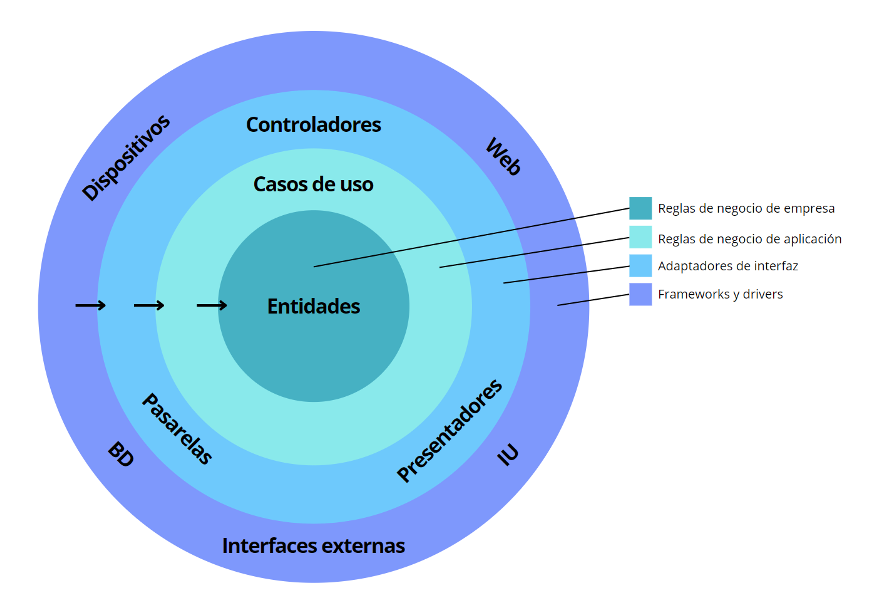
\includegraphics[width=0.7\textwidth]{img/manual/arquitectura_hexagonal.png}
    \caption{Arquitectura hexagonal.} \label{Img:Arquitectura+Hexagonal}
\end{figure} 

La arquitectura hexagonal permite que los sistemas puedan gozar de: a) independencia de frameworks, lo que implica que no depende de una biblioteca de software, sino que más bien puede utilizarlos como herramientas; y b) independencia de la IU, de la base de datos o de cualquier agente externo, lo que implica que el sistema puede ponerse a prueba sin necesidad de cualquiera de estos elementos, u otros, al mismo tiempo que puede cambiar fácilmente de interfaz, de servidor, o de cualquier otro agente externo que necesite. Lo anterior significa que la arquitectura hexagonal ofrece versatilidad al sistema y facilita su adaptabilidad a cualquier entorno de software \cite{book:arquitectura_limpia}. 

En este sentido, las entidades hacen referencia al objeto que establece las reglas del negocio, es decir, las reglas generales que dictan el funcionamiento del sistema. Los casos de uso son reglas de la aplicación más especificas que las anteriores; los adaptadores de interfaz son los encargados de convertir los datos provenientes de la interfaz al formato más conveniente para las dos capas anteriores. En la capa de frameworks y drivers se encuentran herramientas como la base de datos y el framework web, siendo la capa con los detalles menos relevantes que se mantienen en el exterior \cite{book:arquitectura_limpia}. Es importante considerar la regla de la dependencia, la cual estipula que los círculos más externos dependen de los internos y no al contrario, es decir, de adentro hacia afuera cada capa depende de la anterior.

En base a lo precedentemente expuesto amerita explicitar que la selección de la arquitectura hexagonal para el presente proyecto se motivó en que ésta permite el desacoplamiento de la lógica de negocio y las interfaces externas. Esto significa que se puede cambiar la base de datos, interfaz o invocaciones a APIs externas para la misma lógica de negocio, sin alterarla esencialmente. Ello asegura una escalabilidad y mantenibilidad de 
\emph{RedEM} a futuro. Habilitando a modificar, actualizar o reemplazar las partes individuales de la aplicación sin tener que reescribir todo el sistema, me centrarme en la implementación y no en otras capas del mismo. Por último, pero no menos importante, es una arquitectura con la que no tenía experiencia previa y quería desafiarme a aprenderla tanto académicamente como para aplicarla a nivel laboral.


\section{Control de versiones}
\begin{itemize}
\tightlist
\item
  Herramientas consideradas:
  \href{https://git-scm.com/}{Git} y
  \href{https://subversion.apache.org/)}{Subversion (SVN)}.
\item
  Herramienta elegida: \href{https://git-scm.com/}{Git}.
\end{itemize}
Se utilizó Git ya que este ofrece un modelo de ramificación y fusión más avanzado que SVN, lo que permite a los desarrolladores trabajar en paralelo en diferentes características o correcciones de errores sin interferir entre sí \cite{art:pro_git}. Asimismo, SVN consume más recursos a nivel de memoria por tener un sistema de guardado menos eficiente que el de Git. Además, es de considerar que al día de hoy el uso de Git proporciona integración con diferentes herramientas.

\subsection{Gestión del proyecto}
\begin{itemize}
\tightlist
\item
  Herramientas consideradas:
  \href{https://github.com/features/issues}{Github Projects},
  \href{https://trello.com/home)}{Trello} y \href{https://www.atlassian.com/es/software/jira}{Jira}.
\item
  Herramienta elegida: \href{https://www.atlassian.com/es/software/jira)}{Jira}.
\end{itemize}
Las ventajas de JIRA incluyen la capacidad de rastrear y solucionar problemas y tareas de manera eficiente, la personalización de flujos de trabajo y la integración con otras herramientas de Atlassian como Confluence y Bitbucket \cite{art:jira_osman}. De igual forma, posee una interfaz amigable que facilita el seguimiento del proyecto en tiempo real y, a diferencia de otras herramientas, permite tener un flujo de desarrollo de software más adaptado a los estándares de la industria ofreciendo métricas más adecuadas para la evaluación del desarrollo del proyecto, como su velocidad. Asimismo tengo conocimiento de esta herramienta por experiencia laboral.

\subsection{Editor del código}
\begin{itemize}
\tightlist
\item
  Herramientas consideradas:
  \href{https://code.visualstudio.com/}{Visual Studio Code} y 
  \href{https://www.jetbrains.com/go/)}{Goland}.
\item
  Herramienta elegida: \href{https://code.visualstudio.com/}{Visual Studio Code}.
\end{itemize}
Visual Studio Code es un editor de código de fuente abierto, gratuito, y multiplataforma con una gran cantidad de extensiones disponibles, y que se utiliza para desarrollar aplicaciones en una variedad de lenguajes de programación como C, C\#, Java, Python, JavaScript, TypeScript, Golang, entre otros \cite{art:visual_code_flores}. En este sentido, no se requirió de licencia para el editor de código facilitando su uso.

\subsection{Procesador de texto \LaTeX}
\begin{itemize}
\tightlist
\item
  Herramientas consideradas:
  \href{https://www.latex-project.org/}{LATEX} y 
  \href{https://www.microsoft.com/en-ww/microsoft-365/word)}{MS Word}.
\item
  Herramienta elegida: \href{https://www.latex-project.org/}{LATEX}.
\end{itemize}
\LaTeX{} es un lenguaje de marcado utilizado para la creación de documentos científicos y técnicos. En este sentido, se decidió trabajar con \LaTeX{} en el presente proyecto debido a su alta calidad tipográfica, la facilidad para crear fórmulas matemáticas complejas, la capacidad de automatizar la creación de tablas e índices\cite{art:latex}. Fue, asimismo, un desafío ya que no conocía esta herramienta para la elaboración de documentos y decidi acercarme a ella.


\subsection{Calidad del Código}
\begin{itemize}
\tightlist
\item
  Herramientas consideradas:
  \href{https://www.sonarsource.com/products/sonarqube/}{SonarQube} y 
  \href{https://circleci.com/)}{CircleCI}.
\item
  Herramienta elegida: \href{https://www.sonarsource.com/products/sonarqube/}{SonarQube}.
\end{itemize}
SonarQube es una plataforma gratuita de análisis de código abierto que permite evaluar la calidad del código fuente de los proyectos. Esta herramienta está diseñada para identificar y corregir errores de programación, vulnerabilidades de seguridad, patrones de diseño ineficientes y otros problemas comunes que pueden afectar la calidad del código \cite{art:sonarqube_ortega}. Se seleccionó esta herramienta puesto que ofrece informes detallados y personalizables sobre la calidad del código y es compatible con una amplia variedad de lenguajes de programación, como Golang, además de que puede integrarse con Github para obtener información detallada sobre la calidad del código. Asimismo, puede ser instalado en un servidor para ejecutar pruebas, sin pagar licencia por uso, pudiendo ser implementado en proyectos comerciales.


\subsection{Integración Continúa}
\begin{itemize}
\tightlist
\item
  Herramientas consideradas:
  \href{https://www.sonarsource.com/products/sonarqube/}{Github Actions} y 
  \href{https://circleci.com/)}{Jenkins}.
\item
  Herramienta elegida: \href{https://www.sonarsource.com/products/sonarqube/}{Github Actions}.
\end{itemize}
Github Actions es una plataforma que permite automatizar la compilación, prueba y despliegue de un código gracias a su característica de integración y despliegue continuo. Permite hacer despliegues en el servidor, releases, liberar versiones, y tener una mayor cantidad de usuarios por cuenta compartida. Además, tiene una herramienta que permite hacer Gitflow (manejo de branches), lo que facilita la gestión del desarrollo del software. Así, Github Actions permite reducir las acciones requeridas para ejecutar el código a través de la creación de un flujo de trabajo (Canorea, 2021). Se eligió Github Actions por su integración con Github y por el hecho de no necesitar de un hosting propio para ser instalado \cite{art:github_actions}

\subsection{Gestor de base de datos}
\begin{itemize}
\tightlist
\item
  Herramientas consideradas:
  \href{https://tableplus.com/}{TablePlus} y 
  \href{https://www.pgadmin.org/)}{pgAdmin}.
\item
  Herramienta elegida: \href{https://tableplus.com/}{TablePlus}.
\end{itemize}
TablePlus es un software de gestión de bases de datos, que fue seleccionado para el presente proyecto por su interfaz gráfica de usuario intuitiva y fácil de usar, que permite a los usuarios conectarse y administrar múltiples bases de datos de manera eficiente y en una sola aplicación y navegar por bases de datos relacionales de forma cómoda y sencilla \cite{art:tableplus}. Ofrece una serie de características útiles como la de autocompletado código SQL, la búsqueda de texto completo y la vista de schema, que hacen que la gestión de bases de datos sea más eficiente y productiva.

\subsection{Herramientas de diagrama}
\begin{itemize}
\tightlist
\item
  Herramientas consideradas:
  \href{https://draw.io/}{Draw.io} y 
  \href{https://www.lucidchart.com/)}{Lucid Chart}.
\item
  Herramienta elegida: \href{https://draw.io/}{Draw.io}.
\end{itemize}
Es útil para diseñar diagramas de flujo, de procesos, organigramas, diagramas de red, UML, e incluso mapas conceptuales. Posee una interfaz de usuario fácil de manejar y entender basada en la función de arrastrar y soltar, y elementos básicos como flechas, formas, imágenes y demás.
Se eligió esta plataforma para el presente proyecto por su simplicidad y familiaridad con el software. \cite{art:draw_io}

\subsection{Hosting del Proyecto}

\subsubsection{Servidor}
\begin{itemize}
\tightlist
\item
  Herramientas consideradas:
  \href{https://www.digitalocean.com/}{Digital Ocean} y 
  \href{https://aws.amazon.com/es/)}{Amazon AWS}.
\item
  Herramienta elegida: \href{https://www.digitalocean.com/}{Digital Ocean}.
\end{itemize}
Digital Ocean es una plataforma de alojamiento en la nube que ofrece la posibilidad de crear y administrar maquinas virtuales, así como otros servicios relacionados con la infraestructura en la nube; proporciona un entorno seguro y escalable para la implementación de aplicaciones web y móviles \cite{art:digital_ocean}. En este sentido, se eligió Digital Ocean por ser costo-efectivo más conveniente.

\subsubsection{Base de Datos DBaaS (Database as a Service)}
\begin{itemize}
\tightlist
\item
  Herramientas consideradas:
  \href{https://www.digitalocean.com/products/managed-databases}{PostgreSQL Digital Ocean} y 
  \href{https://aws.amazon.com/es/rds/)}{PostgreSQL Amazon}.
\item
  Herramienta elegida:   \href{https://www.digitalocean.com/}{PostgreSQL Digital Ocean}.
\end{itemize}
Digital Ocean también provee alojamiento de base de datos como servicio, con los beneficos de ser altamente escalable, de fácil configuración y mantenimiento, asi como por ofrecer alta disponibilidad dentro de su precio mensual.
Si bien en la comparativa el precio de Amazon AWS era de 24 USD al mes, contra de 33.28 USD de Digital Ocean, se eligió este último a fin de mantener dentro de un mismo ecosistema tanto el hosting como el alojamiento de la base de datos y así no afectará la latencia.
\capitulo{5}{Aspectos relevantes del desarrollo del proyecto}

\subsection{Motivación del proyecto}
La idea del proyecto nace de mi experiencia con una persona cercana que, algunos años atrás, fue diagnosticada con EM, lo que devino en un sinnúmero de desafíos entre los que se encontraba el acceso a una cobertura de salud de calidad. Esto me motivó a indagar sobre la EM, hasta descubrir que Uruguay presenta el índice de prevalencia más alto de Latinoamérica. Más adelante me di cuenta de que existen recursos disponibles en la matriz de protección social que son desconocidos para el público general dada la ausencia de una fuente centralizada de información que reúna toda la data de manera sistematizada y actualizada. 
Ante tal panorama, me planteé el desafío de poner mi bagaje académico y laboral al servicio de la comunidad de pacientes con EM, en mi país, y desarrollar una solución, siendo la elaboración de este trabajo final de grado la oportunidad idónea para ello. Es decir, para crear una herramienta que sirva de apoyo para estas personas y que les ayude a sobreponerse a las dificultades con las que puedan toparse dentro del sistema de salud, así como autogestionar su enfermedad. El plan es que en base al backend desarrollado para este TFG se pueda generar a futuro una aplicación que donaré a la organización sin fines de lucro EMUR (Esclerosis Múltiple Uruguay).

\subsection{Formación necesaria}
Por otro lado, pese a tener una amplia base de conocimientos informáticos, adquiridos tanto de forma académica como por experiencia laboral, fue necesario dedicar una cantidad sustancial de horas al entrenamiento de nuevas habilidades, así como también a la investigación y recolección de información que ayudase al desarrollo del proyecto. En concreto, tuve que profundizar en lo relacionado con la estructura hexagonal, el manejo de Test Automatizados con Postman, la documentación generada con Swagger y las migraciones de bases de datos para versionar cambios sobre las mismas.\\
En cuanto a infraestructura, fue necesario aprender y realizar integraciones continuas en GitHub para así poder desplegar el código mediante la publicación de éste al repositorio, mientras que, en lo referente a la gestión del proyecto, tuve que aprender a manejar la aplicación Jira, para así poder analizar y evaluar la ejecución del proyecto.
En relación con lo anterior, para la arquitectura hexagonal, tomé tres curso relacionados con el tema: “Hexagonal Architecture in Go”, de la plataforma Medium; “Golang. Intermedio”, de la plataforma Platzi; y “Curso de Go. Arquitectura Hexagonal”, de la plataforma Hotmart; mientras que para la integración continua en GitHub recurrí a YouTube y blogs especializados. Para finalizar, es importante mencionar que adquirir todos los conocimientos y habilidades antes mencionadas fue un reto interesante que me permitió ampliar nociones previas y mejorar con ello mi perfil técnico.

\subsection{Contexto Legal}

Este proyecto exigió que me acercara a la legislación uruguaya en relación al manejo de datos personales a nivel nacional.

La normativa vigente se encuentra contenida en: la ley N° 18.331, del año 2008; la ley N° 18.719, del año 2011; el decreto N° 664/008, del año 2008; el decreto N° 414/009, del año 2009.

En lo referente a la ley N° 18.331, el artículo 5 establece los principios generales a los que deben apegarse los responsables, públicos o privados, del manejo de datos personales, siendo estos: legalidad, veracidad, finalidad, previo consentimiento informado, seguridad de los datos, reserva y responsabilidad. Estos principios funcionan también como parámetros a considerar en el diseño de aplicaciones en las que sea necesaria la recolección y manejo de datos de usuarios.
 
A este respecto, según lo establecido en el artículo 8 de dicha ley, el principio de finalidad hace referencia a que los datos recolectados deben ser utilizados única y exclusivamente con los fines previstos y que ello debe serle informado al titular. Es decir, no pueden utilizarse con propósitos distintos a aquellos que motivaron su obtención en un principio. Esto se relaciona a su vez con lo planteado en el artículo 9, sobre el previo consentimiento informado, en donde se expone que el titular debe ser comunicado del manejo que se les dará a sus datos, y de su propósito, para que luego éste decida si consentir o no.

A su vez, el artículo 13, sobre el derecho de información al tratamiento y recolección de datos, profundiza en lo establecido en el artículo 9, e indica que cuando se recolecten datos personales, al titular se le deberá informar, de manera explícita y detallada: el fin con el que se recolectan los datos, quién es el encargado de velar por ellos y manipularlos, cuáles datos son obligatorios y cuáles no, las consecuencias de proporcionar sus datos y qué puede ocurrir si no lo hace, así como si los datos serán transferidos a terceros.

Por otro lado, el artículo 10, sobre la seguridad de los datos, establece que, una vez recopilada la información y almacenada en la base de datos respectiva, el responsable debe adoptar e implementar las medidas de seguridad pertinentes para garantizar la confidencialidad de los datos y la invulnerabilidad de la base de datos. Ello con el fin de evitar la violación a la privacidad, o alteraciones en la información como: adulteración, eliminación, consulta o tratamiento no autorizado, o desviaciones.

En relación con lo anterior, dicha ley, en su capítulo IV sobre los datos especialmente protegidos, establece, en el artículo 19, que los datos relativos a la salud, manejados por entes vinculados al área sanitaria y ciencias de la salud, deberán respetar en todo momento los principios del secreto profesional, procurando proteger la información referente al estado de salud física o mental de los pacientes. Así, este artículo destaca especialmente entre el resto por su relación directa con la temática del presente proyecto y con el backend desarrollado en la que se manejará información sensible sobre las personas con EM.

Esto se ve reforzado por lo expuesto en el artículo 158 de la ley N° 18.719, en donde se indica que las personas, físicas o jurídicas, que intervengan o lleven a cabo actividades relacionadas con la recolección y manejo de datos personales, están en la obligación de preservar el secreto y confidencialidad de la información suministrada por los titulares. Para ello se deben implementar las medidas necesarios que garanticen un óptimo nivel de seguridad e invulnerabilidad de la base de datos en donde se encuentra alojada la información.

Asimismo, volviendo a la ley 18.331, el artículo 15, sobre el derecho de rectificación, actualización, inclusión o supresión, detalla que cada persona, natural o jurídica, que hubiese proporcionado sus datos para cualquier fin, puede solicitar al responsable de la base de datos, en cualquier momento, la rectificación, actualización, inclusión o supresión de la información. Además, establece que, de no hacerse la modificación solicitada por el titular, éste podrá emprender medidas legales contra el responsable en pro del resguardo de sus intereses. Entonces, el backend desarrollador cuenta con los medios necesarios para que los usuarios puedan visualizar y modificar sus datos.

Por último, se tienen los artículos 28 y 29, junto con el decreto N° 664/008, sobre la creación del registro de bases de datos personales, que establecen la obligación que tienen los responsables de las bases de datos de registrarse ante el organismo competente, y de apegarse a la regulación de dicho organismo. Así, se deberá especificar, entre otros datos: identificación de la base de datos y su responsable, naturaleza de los datos que contiene, procedimiento de obtención y tratamiento de la información, medidas de seguridad implementadas, destino de los datos en caso de que sean transferidos a terceros, tiempo de conservación de los datos, y las formas y condiciones en que los titulares pueden acceder y modificar los datos proporcionados.

El decreto N° 414/009 mantiene coherencia con lo anterior. Su artículo 1, establece quién será objeto de protección haciendo referencia a todo aquella persona física que proporcione cualquier tipo de información sobre sí misma. El artículo 2 indica que el régimen de protección de datos personales aplica a las actividades de recolección, registro y tratamiento de información personal. De igual forma, en los artículos 5 y 6 expone lo referente al consentimiento informado para la recolección y tratamiento de datos, de acuerdo con lo cual se le debe informar al titular de la finalidad de los datos y el tipo de actividad que realiza el responsable de los datos. Asimismo, se establece que se le deberá facilitar un medio sencillo, claro y gratuito para que el titular exprese su consentimiento o decline. 

Por otro lado, en su título II, este decreto detalla lo referente a los derechos de los titulares de los datos, señalando el derecho a la modificación de la información proporcionada en cualquier momento, bien sea para rectificar, actualizar, incluir o suprimir datos. En el resto del decreto se mencionan nuevamente las obligaciones del responsable sobre el registro de la base de datos ante el órgano competente, y las características, derechos, deberes y ámbito de acción del órgano de control.

\subsubsection{Protección de datos}

Se implementó una lógica de programación especifica para encriptar los campos de datos “First Name”, “Last Name” y “Profile Image”, evitando asi que ningún usuario administrador, o ningún usuario mal intencionado, logre acceder la información privada de los pacientes con Esclerosis Múltiple. En tanto, el método de encriptación es no determinista, lo que implica que la encriptación es aleatoria, con lo cual si un mismo dato se encripta dos veces la salida generada será distinta cada vez,  lo que dificulta conocer el contenido. Tal encriptación se desarrolló mediante el algoritmo de AES (Advanced Ecryption Standard), en Golang, siguiendo los siguientes pasos:

\begin{itemize}
\tightlist
\item
Primeramente, el texto se convierte en un slice de bytes con el nombre plaintext.

\item Luego, se crea un nuevo bloque de cifrado AES utilizando una clave generada que se aloja en las variables de entorno con el nombre de ENCRYPTION\_KEY.
\item En tercer lugar, se reserva espacio de memoria para la variable ciphertext, donde se almacenará el resultado de dicha encriptación.
\item Seguidamente, se genera un vector de inicialización que se guarda en la variable ciphertext, creada previamente.
\item Después, se crea un flujo de cifrado utilizando el bloque AES y el vector de inicialización para más adelante generar el modo de cifrado CFB (Cipher Feedback).
\item Una vez que se tiene el flujo se procede a cifrar los bytes del texto original y se codifica a base64 usando URL Encoding, para asegurar la el guardado.
\item 
Por último, se devuelve el texto cifrado. 
\end{itemize}

Asimismo, a continuación se detallan los pasos que lleva a cabo el algoritmo para desencriptar:

\begin{itemize}
\tightlist
\item
 Se inicia desencriptando desde base 64.
\item Seguidamente, se crea un bloque de cifrado AES usando la misma clave utilizada para encriptar.
\item Luego, se verifican los datos encriptados para ver si tienen la longitud suficiente para contener un bloque de AES.
\item Después, se extrae el vector de inicialización y se crea el bloque de descifrado, usando AES y el vector de inicialización.
\item Y, por último, se desencriptan los datos y se devuelve el texto desencriptado.
\end{itemize}
\capitulo{6}{Trabajos relacionados}

Con la constante expansión y alcance en crecimiento que tiene la tecnología, cada vez son más los proyectos de software que nacen con la finalidad de resolver los problemas del hombre moderno y satisfacer sus necesidades en los distintos ámbitos de la vida: finanzas, educación, entretenimiento, desarrollo personal, salud. A continuación, se presentan y comparan algunos trabajos con objetivos similares a los planteados para el presente proyecto.

\subsection{Comparativa con otros proyectos}
En esta sección se muestran trabajos realizados hasta la fecha que guardan similitud con el presente proyecto por los objetivos a los que aspiran.

\subsubsection{“Desarrollo de una aplicación móvil para el seguimiento y monitorización en personas con esclerosis múltiple”.}
Se trata de un trabajo de fin de grado para la carrera de ingeniería informática, enfocado en el desarrollo de una aplicación móvil dirigida a pacientes con esclerosis múltiple cuyo propósito fue ofrecer un medio de participación en el control de su enfermedad en conjunto con sus doctores y especialistas, incluyendo funciones como control de medicación, gestión de citas, gestión de documentos, entre otras. Las características de este proyecto se muestran en la tabla ~\ref{tab:comp_APP}, en la columna denominada “EM1”.
\href{https://riunet.upv.es/handle/10251/188415}{Enlace al trabajo}

\subsubsection{“Diseño y desarrollo de una aplicación web para el seguimiento y control de la sintomatología en pacientes con Esclerosis Múltiple (EM)”.}
En este caso se trató de un proyecto presentado en la Universidad Oberta de Catalunya, enfocado en la creación de una aplicación web para pacientes con EM que les permitiese agilizar los tiempos de consulta mediante la gestión de formularios digitales que recojan sus síntomas y demás datos de interés. Las características de este proyecto se muestran en la tabla ~\ref{tab:comp_APP}, en la columna denominada “EM2”.
\href{https://openaccess.uoc.edu/handle/10609/147240}{Enlace al trabajo}

\subsubsection{“Diseño, estudio e implementación de una aplicación móvil para pacientes con esclerosis múltiple”.}
Proyecto desarrollado en la Universidad de Lleida, enfocado en el diseño e implementación de una aplicación móvil que les permitiese a los pacientes con EM llevar un control y seguimiento de su enfermedad y tratamiento mediante el control de eventos, como citas médicas, y comunicación con especialistas. Las características de este proyecto se muestran en la tabla ~\ref{tab:comp_APP}, en la columna denominada “EM3”.
\href{https://repositori.udl.cat/handle/10459.1/69628}{Enlace al trabajo}

\newpage
\begin{table}[]
\centering
\resizebox{\textwidth}{!}{%
\begin{tabular}{|c|c|c|c|c|}
\hline
\rowcolor[HTML]{C0C0C0} 
\color[HTML]{333333} \textbf{Funcionalidad} & \textbf{EM1} & \textbf{EM2} & \textbf{EM3} & \textbf{RedEM} \\
\rowcolor[HTML]{FFFFFF} \textbf{Registro de usuario} & \textbf{\checkmark} & \textbf{\checkmark} & \textbf{\checkmark} & \textbf{\checkmark}\\
\rowcolor[HTML]{FFFFFF} \textbf{Chatbot} & \textbf{} & \textbf{} & \textbf{} & \textbf{\checkmark}\\
\rowcolor[HTML]{FFFFFF} \textbf{Consejos, noticias o artículos de interés} & \textbf{\checkmark} & \textbf{} & \textbf{} & \textbf{\checkmark}\\
\rowcolor[HTML]{FFFFFF} \textbf{Diario de control de síntomas y medicación} &  \textbf{\checkmark} & \textbf{\checkmark} & \textbf{\checkmark} & \textbf{\checkmark}\\
\rowcolor[HTML]{FFFFFF} \textbf{Calendario para citas médicas} &  \textbf{\checkmark} & \textbf{} & \textbf{\checkmark} & \textbf{\checkmark}\\
\rowcolor[HTML]{FFFFFF} \textbf{Gráficos de seguimiento} &  \textbf{} & \textbf{\checkmark} & \textbf{} & \textbf{}\\
\rowcolor[HTML]{FFFFFF} \textbf{Planes de ejercicio físico} &  \textbf{\checkmark} & \textbf{} & \textbf{\checkmark} & \textbf{\checkmark}\\
\rowcolor[HTML]{FFFFFF} \textbf{Sistema de alarmas y recordatorios} &  \textbf{\checkmark} & \textbf{} & \textbf{\checkmark} & \textbf{\checkmark}\\
\rowcolor[HTML]{FFFFFF} \textbf{Guardar y compartir informes médicos} &  \textbf{\checkmark} & \textbf{\checkmark} & \textbf{} & \textbf{\checkmark}\\
\rowcolor[HTML]{FFFFFF} \textbf{Recetas alimenticias} &  \textbf{} & \textbf{} & \textbf{} & \textbf{\checkmark}\\
\rowcolor[HTML]{FFFFFF} \textbf{Preguntas y respuestas} &  \textbf{} & \textbf{} & \textbf{} & \textbf{\checkmark}\\
\rowcolor[HTML]{FFFFFF} \textbf{Mapa de servicios} &  \textbf{} & \textbf{} & \textbf{} & \textbf{\checkmark}\\
\rowcolor[HTML]{FFFFFF} \textbf{Clima} &  \textbf{} & \textbf{} & \textbf{} & \textbf{\checkmark}\\
\rowcolor[HTML]{FFFFFF} \textbf{Comparación y análisis de resultados} &  \textbf{} & \textbf{} & \textbf{} & \textbf{\checkmark}\\
\hline
\end{tabular}}%
\caption{Comparativa de aplicaciones de Esclerosis Múltiple.}
\label{tab:comp_APP}
\end{table}

\subsubsection{Principales fortalezas de \emph{RedEM}}
\begin{itemize}
\tightlist
\item
Proporciona al usuario recetas alimenticias, sección de preguntas y respuestas, e información del clima para el cuidado del paciente. 
\item 
Ofrece un mapa de servicios que le permite al paciente acceder a servicios de terceros que pueden ayudarle en situaciones concretas.
\item 
Dispone de un chatbot con el cual los pacientes podrán interactuar accediendo a información fidedigna de la Asociación para poder evacuar sus dudas ágilmente.
\item
Proporciona información actualizada, consejos y noticias referentes a la EM.
\item 
\emph{RedEM} operará utilizando un servidor que le permite atender a múltiples requests de forma simultánea sin que afecte su rendimiento.
\end{itemize}

\capitulo{7}{Conclusiones y Líneas de trabajo futuras}


\subsection{Conclusiones}
La confección del presente TFG me ha permitido robustecer algunos conocimientos previos, así como también acercarme a técnicas y herramientas de las que manejaba vagas ideas y que me fueron seduciendo conforme el desarrollo del proyecto avanzaba. Asimismo, poner mi bagaje académico al servicio de una comunidad me interpeló profundamente confirmándome que cada persona puede configurarse como un agente de cambios positivos para la sociedad toda.

A continuación, detallo algunas de las conclusiones a las que he arribado a partir de este significativo proyecto en mi trayectoria académica-profesional.

\begin{itemize}
\item A través de la combinación de múltiples entornos de desarrollo, como Golang y Python, y diversas plataformas, se logró crear el backend y el chatbot para una futura aplicación que integra una serie de funciones que pretenden colaborar a la mejora de la calidad de vida de las personas afectadas por la EM.

\item Por tratarse del backend de una aplicación que será destinada a una organización sin fines de lucro, se puso especial énfasis en el ámbito económico procurando minimizar los costes de desarrollo. Ello implicó el uso de software y plataformas en su mayoría gratuitos sin afectar la funcionalidad o sacrificar bondades, lo que reafirma que es posible crear soluciones costo-efectivas.

\item Por otro lado, la tolerancia a alta concurrencia sin provocar fallos, así como el exiguo espacio de memoria requerido para el funcionamiento del backend, dieron como resultado una solución robusta que ofrece una buena experiencia de usuario.

\item Amerita explicitar que el desarrollo de la aplicación móvil como tal insumirá tiempo y recursos, desafiándome a concretarla para poder cumplir con mi propósito de donarla a EMUR.

\item Por último pero no menos importante, en lo referente a los objetivos personales, el desarrollo del proyecto supuso un proceso de aprendizaje continuo en el que pude adquirir nuevas habilidades tanto en el ámbito de la programación y desarrollo de software, como en el metodológico concerniente a la elaboración de esta memoria y a la documentación formal requerida.

\end{itemize}


\subsection{Lineas de trabajo a futuro}

\begin{itemize}
\item Se deberá desarrollar la aplicación móvil tanto para los sistemas operativos Android como iOS con el fin de llegar a la mayor cantidad de usuarios posibles, para lo cual se empleará el lenguaje Flutter debido a la portabilidad que el mismo ofrece.

\item Además, se separará la capa de operaciones del administrador de la del usuario en 2 microservicios diferentes, para discriminar la responsabilidad y potenciar la escalibilidad.

\item En lo referente a la escalabilidad, adicionalmente, se utilizará el orquestador de contenedores llamado Kubernetes, para mejorar el flujo de despliegue ante la posible alta concurrencia.

\item Se desarrollará un frontend para el backend ya creado con el fin de que los usuarios administradores puedan gestionar contenidos con mayor facilidad y mejor experiencia de usuario.

\item Se invertirán esfuerzos en continuar entrenando el chatbot con diferentes fuentes de datos para que éste brinde respuestas con mayor, más fehaciente y precisa información referente a la EM.

\item  Para optimizar el chatbot, además, se utilizará el alojamiento Pinecode para almacenar los vectores, logrando así una búsqueda más eficiente y célere.
\end{itemize}


\bibliographystyle{plain}
\bibliography{bibliografia}

\end{document}
